\documentclass[10pt]{beamer}

% Tema Limpo e Profissional (Idêntico à Aula 20)
\usetheme{Madrid}
\usecolortheme{whale}

% Pacotes Essenciais
\usepackage[utf8]{inputenc}
\usepackage[T1]{fontenc}
\usepackage[portuguese]{babel}
\usepackage{graphicx}
\usepackage{booktabs}
\usepackage{amsmath}
\usepackage{amssymb}
\usepackage{listings}
\usepackage{xcolor}

% Configuracoes de Codigo (Python)
\lstset{
    language=Python,
    basicstyle=\ttfamily\scriptsize,
    keywordstyle=\color{blue}\bfseries,
    stringstyle=\color{red!80!black},
    commentstyle=\color{green!60!black},
    breaklines=true,
    showstringspaces=false,
    tabsize=4
}

% Metadados da Apresentacao
\title[IFCE Tauá - Engenharia de Software]{Aula 21: Diagrama de Classes e Diagrama de Atividades}
\subtitle{Fundamentação Estrutural e Comportamental baseada nos Capítulos 4 e 10 (Gilleanes Guedes)}
\author[Prof. Reginaldo Fernandes]{Prof. Reginaldo Pereira Fernandes\texorpdfstring{\\ \small{Técnico em Informática para Internet}}{}}
\institute[IFCE]{Instituto Federal do Ceará -- Campus Tauá}
\date{\today}

\begin{document}

% -----------------------------------------------------------------------------
% SLIDE 1: Capa
% -----------------------------------------------------------------------------
\begin{frame}
    \titlepage
\end{frame}

% -----------------------------------------------------------------------------
% SLIDE 2: Sumario
% -----------------------------------------------------------------------------
\begin{frame}{Sumário da Aula}
    \tableofcontents
\end{frame}

% =============================================================================
\section{Aprofundamento no Diagrama de Classes (Cap. 4)}
% =============================================================================

% -----------------------------------------------------------------------------
% SLIDE 3: Do Caso de Uso à Estrutura Interna
% -----------------------------------------------------------------------------
\begin{frame}{Do Caso de Uso à Estrutura Interna do Sistema}
    \begin{columns}
        \begin{column}{0.55\textwidth}
            \textbf{A Transição da Análise para o Projeto:}
            \begin{itemize}
                \item Na \textbf{Aula 20 (Cap. 3)}, modelamos o sistema como uma \textit{``caixa-preta''} através dos Casos de Uso.
                \item Na \textbf{Aula 21 (Cap. 4)}, abrimos a caixa para projetar o alicerce estático com o \textbf{Diagrama de Classes}.
            \end{itemize}
            \vspace{0.2cm}
            \textbf{Papel Central do Diagrama de Classes:}
            \begin{itemize}
                \item É o diagrama estrutural mais importante da UML;
                \item Base direta para a geração de código-fonte OO e para o esquema de banco de dados.
            \end{itemize}
        \end{column}
        \begin{column}{0.45\textwidth}
            \begin{block}{Níveis de Modelagem (Guedes)}
                \begin{itemize}
                    \item \textbf{Modelo Conceitual:} Fase de análise; foca nas classes e atributos do domínio do problema.
                    \item \textbf{Modelo de Domínio:} Fase de projeto; detalha assinaturas de métodos, navegabilidade e interfaces da solução.
                \end{itemize}
            \end{block}
        \end{column}
    \end{columns}
\end{frame}

% -----------------------------------------------------------------------------
% SLIDE 4: Atributos, Assinaturas e Valores Derivados (Fig. 4.1, 4.2, 4.3)
% -----------------------------------------------------------------------------
\begin{frame}{Detalhamento de Atributos e Assinaturas de Operações}
    \begin{columns}
        \begin{column}{0.52\textwidth}
            \textbf{Sintaxe de Atributos (Fig. 4.3):}
            \begin{itemize}
                \item \scriptsize\texttt{vis [/] nome: tipo [mult] = val \{prop\}}
                \item \footnotesize\textbf{Barra (\texttt{/}):} Indica \textbf{atributo derivado} (calculado dinamicamente, ex.: \texttt{/saldoConta}).
                \item \textbf{Multiplicidade \texttt{[0..1]}:} Indica atributo opcional (ex.: \texttt{/fechamentoConta}).
                \item \textbf{Valor Inicial:} Atribuído na instanciação (ex.: \texttt{situacaoConta: int = 1}).
            \end{itemize}
            \vspace{0.05cm}
            \textbf{Assinatura de Operações (Fig. 4.2):}
            \begin{itemize}
                \item \footnotesize Especifica parâmetros \texttt{(nome: Tipo)} e retorno \texttt{: TipoRetorno}.
            \end{itemize}
        \end{column}
        \begin{column}{0.48\textwidth}
            \centering
            \textbf{Atributos Detalhados (Fig. 4.3):}\\[0.08cm]
            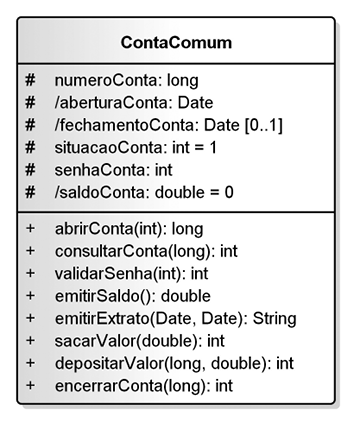
\includegraphics[width=\columnwidth,height=0.31\textheight,keepaspectratio]{imagens/Fig4.3.png}\\[0.12cm]
            \textbf{Assinaturas de Métodos (Fig. 4.2):}\\[0.08cm]
            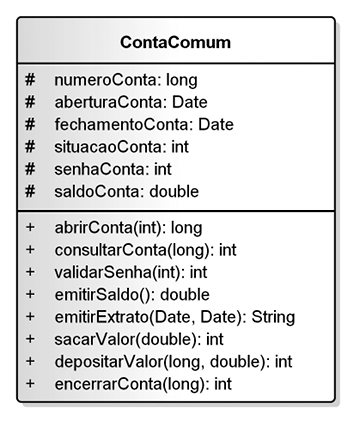
\includegraphics[width=\columnwidth,height=0.31\textheight,keepaspectratio]{imagens/Fig4.2.png}
        \end{column}
    \end{columns}
\end{frame}

% -----------------------------------------------------------------------------
% SLIDE 5: Associação Unária ou Reflexiva e Papéis (Fig. 4.4 e 4.5)
% -----------------------------------------------------------------------------
\begin{frame}{Associação Unária (Reflexiva) e Definição de Papéis}
    \begin{columns}
        \begin{column}{0.52\textwidth}
            \textbf{Associação Unária / Reflexiva (4.4):}
            \begin{itemize}
                \item Ocorre quando instâncias de uma classe relacionam-se com outras instâncias da \textbf{mesma classe}.
                \item Exemplo clássico: um \texttt{Funcionario} gerencia vários outros objetos \texttt{Funcionario}.
            \end{itemize}
            \vspace{0.15cm}
            \textbf{Papéis nas Extremidades (4.5):}
            \begin{itemize}
                \item Esclarecem a função exercida por cada objeto no vínculo:
                \begin{itemize}
                    \item Extremidade \texttt{1}: papel \texttt{+chefe};
                    \item Extremidade \texttt{*}: papel \texttt{+subordinados}.
                \end{itemize}
            \end{itemize}
        \end{column}
        \begin{column}{0.48\textwidth}
            \centering
            \textbf{Associação Reflexiva (Fig. 4.4):}\\[0.1cm]
            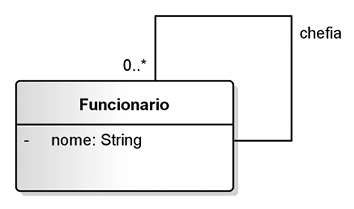
\includegraphics[width=0.88\columnwidth,height=0.32\textheight,keepaspectratio]{imagens/Fig4.4.png}\\[0.15cm]
            \textbf{Com Papéis Explícitos (Fig. 4.5):}\\[0.1cm]
            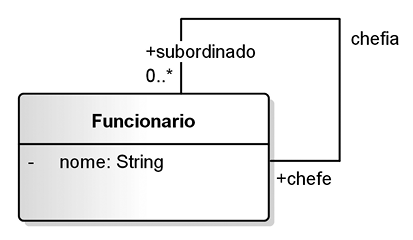
\includegraphics[width=0.92\columnwidth,height=0.32\textheight,keepaspectratio]{imagens/Fig4.5.png}
        \end{column}
    \end{columns}
\end{frame}

% -----------------------------------------------------------------------------
% SLIDE 6: Associação Binária, Multiplicidade e Navegabilidade (Fig. 4.6, 4.7, 4.8)
% -----------------------------------------------------------------------------
\begin{frame}{Associação Binária, Multiplicidade e Navegabilidade}
    \begin{columns}
        \begin{column}{0.52\textwidth}
            \textbf{Associação Binária (4.6):}
            \begin{itemize}
                \item Conecta objetos de duas classes distintas (ex.: um \texttt{Socio} registra \texttt{0..*} objetos \texttt{Dependente}).
            \end{itemize}
            \vspace{0.1cm}
            \textbf{Navegabilidade (4.7):}
            \begin{itemize}
                \item Representada por uma \textbf{seta aberta} indicando o sentido em que as mensagens e referências trafegam (\texttt{Socio $\longrightarrow$ Dependente}).
            \end{itemize}
            \vspace{0.1cm}
            \textbf{Fim de Associação Possuída (4.8):}
            \begin{itemize}
                \item Pequeno ponto cheio (\textit{class-owned end}) indicando que o papel torna-se um atributo de referência na classe origem.
            \end{itemize}
        \end{column}
        \begin{column}{0.48\textwidth}
            \centering
            \textbf{Navegabilidade (Fig. 4.7):}\\[0.1cm]
            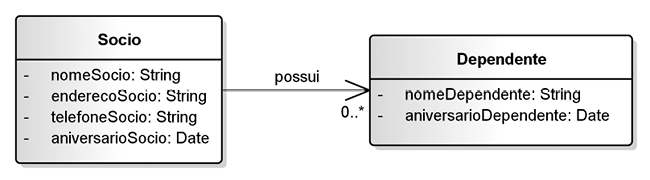
\includegraphics[width=\columnwidth,height=0.32\textheight,keepaspectratio]{imagens/Fig4.7.png}\\[0.15cm]
            \textbf{Class-Owned End (Fig. 4.8):}\\[0.1cm]
            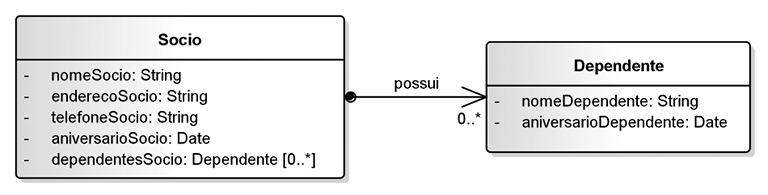
\includegraphics[width=\columnwidth,height=0.34\textheight,keepaspectratio]{imagens/Fig4.8.png}
        \end{column}
    \end{columns}
\end{frame}

% -----------------------------------------------------------------------------
% SLIDE 7: Associação Ternária ou N-ária (Fig. 4.9)
% -----------------------------------------------------------------------------
\begin{frame}{Associação Ternária ou N-ária}
    \begin{columns}
        \begin{column}{0.48\textwidth}
            \textbf{Quando utilizar?}
            \begin{itemize}
                \item Conecta simultaneamente objetos de \textbf{três ou mais classes} através de um \textbf{losango centralizador}.
                \item Exemplo acadêmico (Fig. 4.9): o vínculo entre \texttt{Professor}, \texttt{Turma} e \texttt{SalaDeAula}.
                \item Um professor leciona para $1..*$ turmas utilizando $1..*$ salas (ex.: sala teórica e laboratório).
            \end{itemize}
            \vspace{0.1cm}
            \begin{alertblock}{Recomendação Prática}
                Use apenas quando o vínculo for indivisível entre as 3 classes; caso contrário, prefira uma classe intermediária.
            \end{alertblock}
        \end{column}
        \begin{column}{0.52\textwidth}
            \centering
            \textbf{Associação Ternária (Figura 4.9):}\\[0.15cm]
            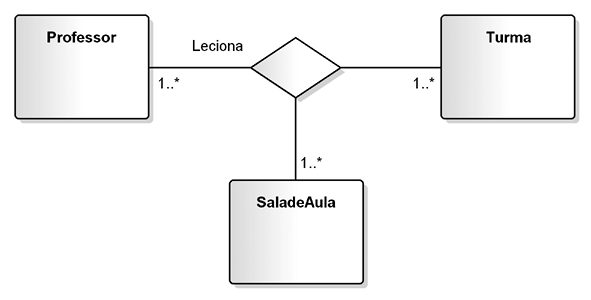
\includegraphics[width=\columnwidth,height=0.68\textheight,keepaspectratio]{imagens/Fig4.9.png}
        \end{column}
    \end{columns}
\end{frame}

% -----------------------------------------------------------------------------
% SLIDE 8: Agregação: Relação Todo-Parte Fraca (Fig. 4.10)
% -----------------------------------------------------------------------------
\begin{frame}{Relacionamento Todo-Parte: Agregação ($\lozenge$)}
    \begin{columns}
        \begin{column}{0.52\textwidth}
            \textbf{Conceito de Agregação:}
            \begin{itemize}
                \item Demonstra que as informações de um \textbf{Objeto-Todo} são complementadas por um ou mais \textbf{Objetos-Parte}.
                \item Símbolo gráfico: \textbf{losango vazio ($\lozenge$)} posicionado junto ao Objeto-Todo.
            \end{itemize}
            \vspace{0.15cm}
            \textbf{Independência de Ciclo de Vida:}
            \begin{itemize}
                \item Vínculo mais fraco: os objetos-parte podem ser compartilhados e \textbf{continuam existindo} mesmo que o objeto-todo seja excluído.
            \end{itemize}
        \end{column}
        \begin{column}{0.48\textwidth}
            \centering
            \textbf{Agregação na UML (Figura 4.10):}\\[0.15cm]
            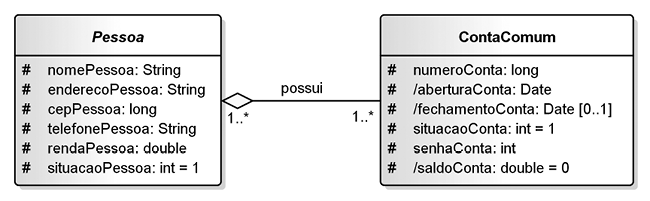
\includegraphics[width=\columnwidth,height=0.55\textheight,keepaspectratio]{imagens/Fig4.10.png}\\[0.1cm]
            \scriptsize \texttt{Pessoa} (Todo) agrega \texttt{ContaComum} (Parte) em relação $1..*$ para $1..*$.
        \end{column}
    \end{columns}
\end{frame}

% -----------------------------------------------------------------------------
% SLIDE 9: Composição: Relação Todo-Parte Forte (Fig. 4.11)
% -----------------------------------------------------------------------------
\begin{frame}{Relacionamento Todo-Parte Forte: Composição ($\blacklozenge$)}
    \begin{columns}
        \begin{column}{0.52\textwidth}
            \textbf{Conceito de Composição:}
            \begin{itemize}
                \item Variação estrita da agregação com \textbf{vínculo forte e exclusivo} entre o Todo e suas Partes.
                \item Símbolo gráfico: \textbf{losango preenchido ($\blacklozenge$)} ao lado do Objeto-Todo.
            \end{itemize}
            \vspace{0.15cm}
            \textbf{Regras Fundamentais:}
            \begin{enumerate}
                \item Cada instância-parte pertence a \textbf{um único} objeto-todo por vez (multiplicidade \texttt{1} no lado do Todo);
                \item Se o objeto-todo for destruído, todas as suas partes são \textbf{destruídas em cascata}!
            \end{enumerate}
        \end{column}
        \begin{column}{0.48\textwidth}
            \centering
            \textbf{Composição na UML (Figura 4.11):}\\[0.15cm]
            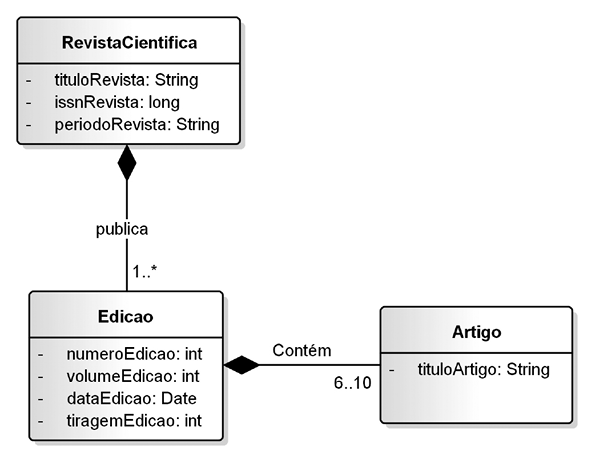
\includegraphics[width=\columnwidth,height=0.65\textheight,keepaspectratio]{imagens/Fig4.11.png}\\[0.05cm]
            \scriptsize \texttt{RevistaCientifica} $\blacklozenge\to$ \texttt{Edicao} $\blacklozenge\to$ \texttt{Artigo}.
        \end{column}
    \end{columns}
\end{frame}

% -----------------------------------------------------------------------------
% SLIDE 10: Generalização/Especialização e Classes Abstratas (Fig. 4.12)
% -----------------------------------------------------------------------------
\begin{frame}{Generalização, Especialização e Classes Abstratas}
    \begin{columns}
        \begin{column}{0.48\textwidth}
            \textbf{Herança no Diagrama de Classes:}
            \begin{itemize}
                \item Seta triangular vazia apontando da subclasse para a superclasse.
                \item \textbf{Classe Abstrata:} Não pode ser instanciada diretamente; seu nome é grafado em \textit{itálico} (ex.: \textit{\texttt{Pessoa}} na Fig. 4.12).
                \item \textbf{Classes Concretas:} Herdam atributos/métodos e instanciam objetos (ex.: \texttt{PessoaFisica}, \texttt{PessoaJuridica}, \texttt{ContaEspecial}, \texttt{ContaPoupanca}).
            \end{itemize}
        \end{column}
        \begin{column}{0.52\textwidth}
            \centering
            \textbf{Hierarquia Bancária (Figura 4.12):}\\[0.1cm]
            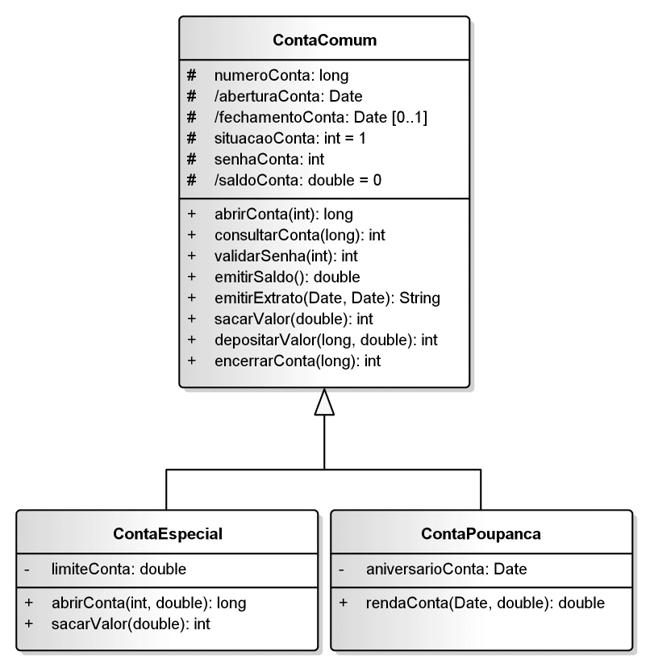
\includegraphics[width=\columnwidth,height=0.72\textheight,keepaspectratio]{imagens/Fig4.12.png}
        \end{column}
    \end{columns}
\end{frame}

% -----------------------------------------------------------------------------
% SLIDE 11: Classe Associativa vs. Classe Intermediária (Fig. 4.13 e 4.14)
% -----------------------------------------------------------------------------
\begin{frame}{Classe Associativa vs. Classe Intermediária}
    \begin{columns}
        \begin{column}{0.5\textwidth}
            \textbf{1. Classe Associativa (Fig. 4.13):}
            \begin{itemize}
                \item Ligada por linha tracejada ao meio de uma associação (geralmente \texttt{*} para \texttt{*}).
                \item Armazena atributos que pertencem \textbf{ao vínculo} (ex.: \texttt{papelAtorFilme}).
                \item \textbf{Restrição:} Admite apenas \textbf{uma única ocorrência} para cada par de objetos $(a, f)$.
            \end{itemize}
            \centering
            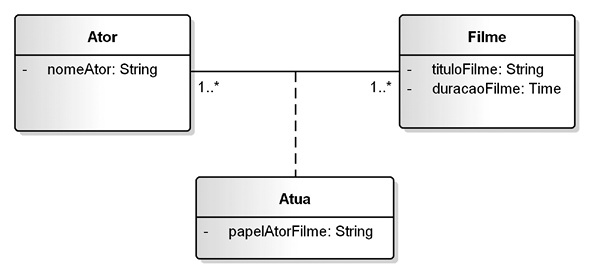
\includegraphics[width=0.92\columnwidth,height=0.35\textheight,keepaspectratio]{imagens/Fig4.13.png}
        \end{column}
        \begin{column}{0.5\textwidth}
            \textbf{2. Classe Intermediária (Fig. 4.14):}
            \begin{itemize}
                \item Quando o mesmo par de objetos pode se relacionar \textbf{múltiplas vezes} (ex.: um ator interpreta dois papéis no mesmo filme).
                \item Substitui-se a ligação tracejada por uma \textbf{classe intermediária normal} com associações \texttt{1} para \texttt{1..*}.
            \end{itemize}
            \centering
            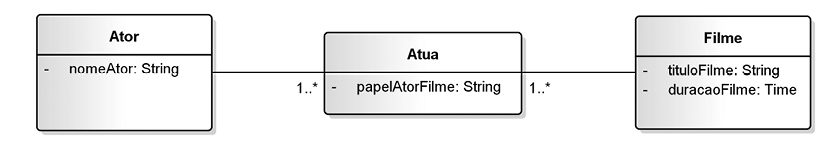
\includegraphics[width=0.92\columnwidth,height=0.35\textheight,keepaspectratio]{imagens/Fig4.14.png}
        \end{column}
    \end{columns}
\end{frame}

% -----------------------------------------------------------------------------
% SLIDE 12: Associação Qualificada e Dependência (Fig. 4.15 e 4.16)
% -----------------------------------------------------------------------------
\begin{frame}{Associação Qualificada e Relacionamento de Dependência}
    \begin{columns}
        \begin{column}{0.5\textwidth}
            \textbf{Associação Qualificada (4.15):}
            \begin{itemize}
                \item Utiliza um atributo chave (qualificador em pequeno retângulo, ex.: \texttt{numeroConta}) para indexar uma coleção.
                \item Reduz a multiplicidade de \texttt{1..*} para \texttt{1} na busca direta de uma instância.
            \end{itemize}
            \centering
            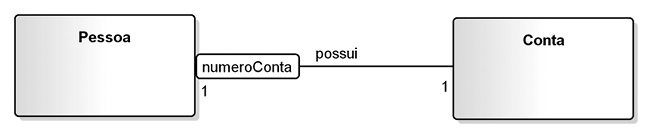
\includegraphics[width=0.95\columnwidth,height=0.36\textheight,keepaspectratio]{imagens/Fig4.15.png}
        \end{column}
        \begin{column}{0.5\textwidth}
            \textbf{Dependência (\texttt{- - ->}) (4.16):}
            \begin{itemize}
                \item Relação cliente/fornecedor fraca e transitória (ex.: classe \texttt{Pedido} recebe ou usa um objeto \texttt{Pagamento} como parâmetro de método).
                \item Linha tracejada com seta aberta apontando para o fornecedor.
            \end{itemize}
            \centering
            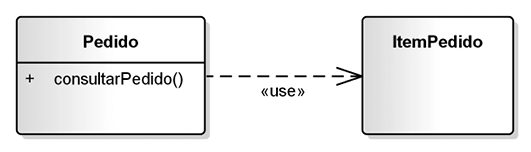
\includegraphics[width=0.95\columnwidth,height=0.36\textheight,keepaspectratio]{imagens/Fig4.16.png}
        \end{column}
    \end{columns}
\end{frame}

% -----------------------------------------------------------------------------
% SLIDE 13: Realização e Interfaces Fornecidas/Requeridas (Fig. 4.18 e 4.22)
% -----------------------------------------------------------------------------
\begin{frame}{Realização e Interfaces (\texttt{<<interface>>})}
    \begin{columns}
        \begin{column}{0.52\textwidth}
            \textbf{Realização de Contrato (Fig. 4.18):}
            \begin{itemize}
                \item Uma interface define assinaturas de operações sem implementá-las (\texttt{+quitarPedido()}).
                \item Classes concretas (\texttt{PagamentoBoleto}, \texttt{PagamentoCartaoCredito}) \textbf{realizam} a interface (linha tracejada com triângulo vazio).
            \end{itemize}
            \centering
            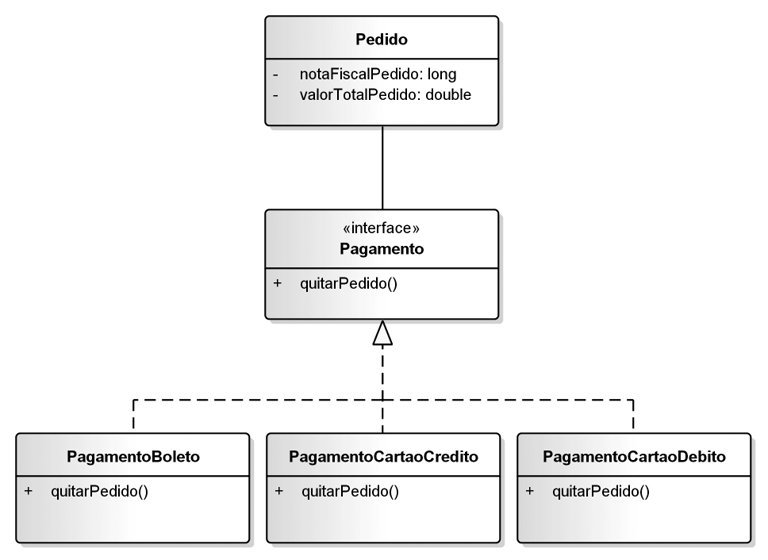
\includegraphics[width=0.95\columnwidth,height=0.41\textheight,keepaspectratio]{imagens/Fig4.18.png}
        \end{column}
        \begin{column}{0.48\textwidth}
            \textbf{Notação Pirulito/Soquete (4.22):}
            \begin{itemize}
                \item \textbf{Interface Fornecida ($\multimap$):} Círculo fechado (serviço provido pela classe).
                \item \textbf{Interface Requerida ($\subset$):} Semicírculo (serviço consumido pela classe através de uma Porta).
            \end{itemize}
            \vspace{0.1cm}
            \centering
            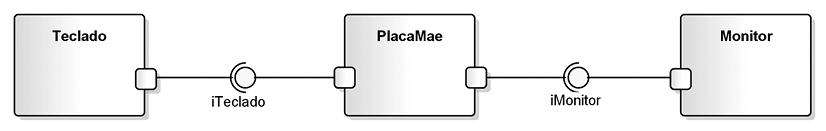
\includegraphics[width=0.95\columnwidth,height=0.34\textheight,keepaspectratio]{imagens/Fig4.22.png}
        \end{column}
    \end{columns}
\end{frame}

% -----------------------------------------------------------------------------
% SLIDE 14: Restrições, Atributos Estáticos e OCL (Fig. 4.25, 4.28, 4.29)
% -----------------------------------------------------------------------------
\begin{frame}{Restrições, Atributos Estáticos e Linguagem OCL}
    \begin{columns}
        \begin{column}{0.52\textwidth}
            \textbf{Propriedades e Restrições entre Chaves:}
            \begin{itemize}
                \item \textbf{\texttt{\{readOnly\}} (4.28):} Atributo somente leitura após criação (ex.: \texttt{numeroConta}).
                \item \textbf{Membro Estático (4.29):} Grafado \underline{sublinhado}; seu valor é compartilhado por toda a classe (ex.: \underline{\texttt{tomLigacao}}).
                \item \textbf{\texttt{\{ordered\}}, \texttt{\{unique\}}, \texttt{\{xor\}}:} Regras sobre coleções e associações.
            \end{itemize}
            \vspace{0.1cm}
            \textbf{OCL (Object Constraint Language) (4.25):}
            \begin{itemize}
                \item Especifica invariantes formais sem ambiguidade: \texttt{context PessoaFisica inv: self.idade >= 18}.
            \end{itemize}
        \end{column}
        \begin{column}{0.48\textwidth}
            \centering
            \textbf{Restrição OCL (Fig. 4.25):}\\[0.08cm]
            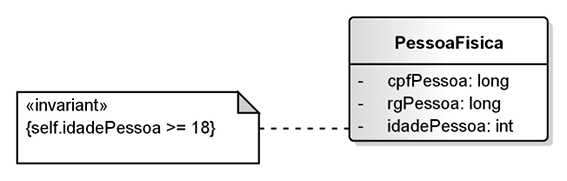
\includegraphics[width=0.95\columnwidth,height=0.32\textheight,keepaspectratio]{imagens/Fig4.25.png}\\[0.12cm]
            \textbf{Atributo Estático Sublinhado (Fig. 4.29):}\\[0.08cm]
            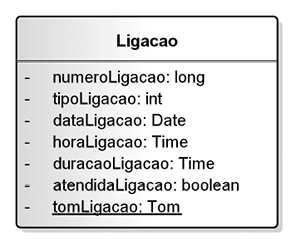
\includegraphics[width=0.82\columnwidth,height=0.34\textheight,keepaspectratio]{imagens/Fig4.29.png}
        \end{column}
    \end{columns}
\end{frame}

% -----------------------------------------------------------------------------
% SLIDE 15: Estereótipos: Enumeração e Arquitetura MVC/ECB (Fig. 4.38, 4.44, 4.47)
% -----------------------------------------------------------------------------
\begin{frame}{Estereótipos de Classes: Enumeração e Padrão MVC/ECB}
    \begin{columns}
        \begin{column}{0.5\textwidth}
            \textbf{1. \texttt{<<enumeration>>} (Fig. 4.38):}
            \begin{itemize}
                \item Lista o domínio fechado de valores literais válidos para um atributo (ex.: \texttt{SituacaoExemplar}: \texttt{disponivel}, \texttt{emprestado}, \texttt{atrasado}).
            \end{itemize}
            \centering
            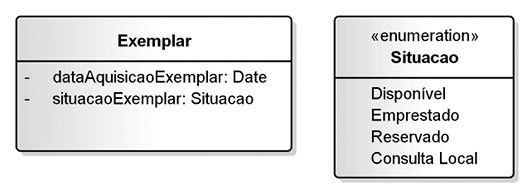
\includegraphics[width=0.95\columnwidth,height=0.36\textheight,keepaspectratio]{imagens/Fig4.38.png}
        \end{column}
        \begin{column}{0.5\textwidth}
            \textbf{2. Camadas MVC / ECB (4.44 e 4.47):}
            \begin{itemize}
                \item \textbf{\texttt{<<boundary>>} (Fronteira/Visão):} Telas e interfaces com usuário;
                \item \textbf{\texttt{<<control>>} (Controle):} Coordena casos de uso;
                \item \textbf{\texttt{<<entity>>} (Entidade/Modelo):} Objetos de negócio persistentes.
            \end{itemize}
            \centering
            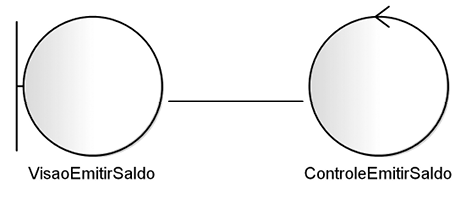
\includegraphics[width=0.92\columnwidth,height=0.28\textheight,keepaspectratio]{imagens/Fig4.44.png}\\[0.08cm]
            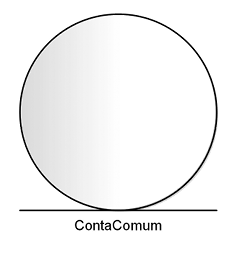
\includegraphics[width=0.78\columnwidth,height=0.18\textheight,keepaspectratio]{imagens/Fig4.47.png}
        \end{column}
    \end{columns}
\end{frame}

% -----------------------------------------------------------------------------
% SLIDE 16: Estudo de Caso: Modelo de Domínio Bancário Completo (Fig. 4.51)
% -----------------------------------------------------------------------------
\begin{frame}{Estudo de Caso: Modelo de Domínio do Sistema Bancário}
    \centering
    \textbf{Diagrama de Classes - Modelo de Domínio (Figura 4.51 do Livro):}\\[0.1cm]
    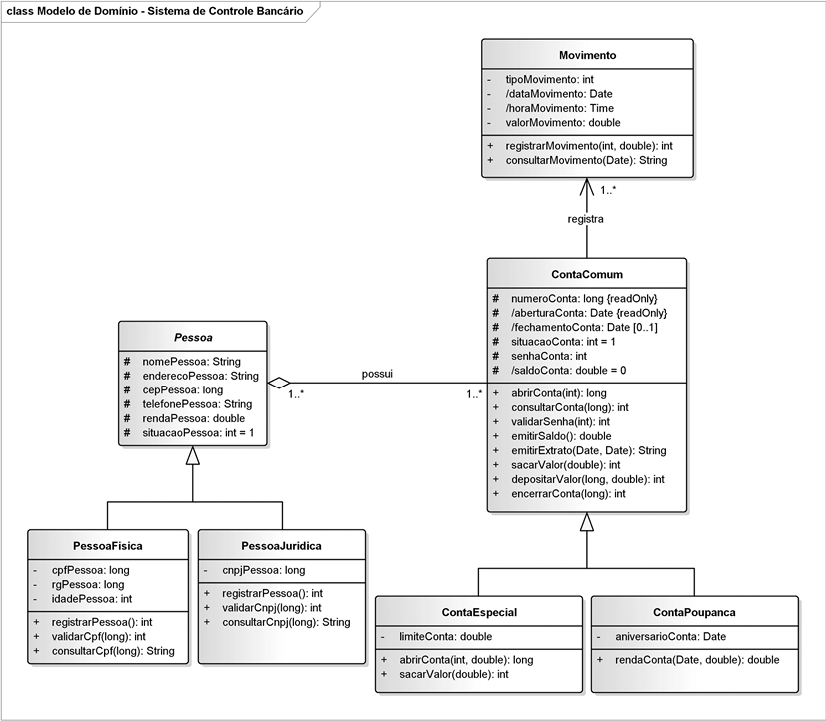
\includegraphics[width=0.94\textwidth,height=0.73\textheight,keepaspectratio]{imagens/Fig4.51.png}\\[0.08cm]
    \scriptsize Reúne classe abstrata (\textit{Pessoa}), herança, agregação ($\lozenge$), navegabilidade, atributos derivados (\texttt{/}) e \texttt{\{readOnly\}}.
\end{frame}

% -----------------------------------------------------------------------------
% SLIDE 17: Estudo de Caso Web: Sistema de Leilão Via Internet (Fig. 4.72)
% -----------------------------------------------------------------------------
\begin{frame}{Estudo de Caso Web: Sistema de Leilão Via Internet}
    \centering
    \textbf{Modelo de Domínio para Leilão Online (Figura 4.72 do Livro):}\\[0.1cm]
    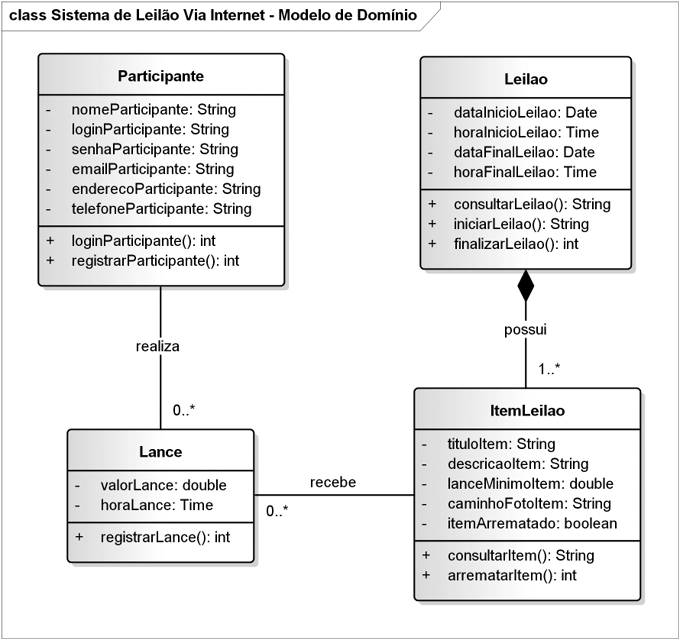
\includegraphics[width=0.92\textwidth,height=0.73\textheight,keepaspectratio]{imagens/Fig4.72.png}\\[0.08cm]
    \scriptsize Observe a Composição ($\blacklozenge$) entre \texttt{Leilao} e \texttt{ItemLeilao} e a classe intermediária \texttt{Lance} entre \texttt{Participante} e \texttt{ItemLeilao}.
\end{frame}

% -----------------------------------------------------------------------------
% SLIDE 18: Mapeamento Objeto-Relacional e Padrões Repository/DAO
% -----------------------------------------------------------------------------
\begin{frame}{Persistência, Mapeamento Relacional e Repository/DAO}
    \begin{columns}
        \begin{column}{0.5\textwidth}
            \textbf{Mapeamento em Tabelas (\texttt{<<Table>>}):}
            \begin{itemize}
                \item \textbf{1:N (Fig. 4.59):} Chave estrangeira (\texttt{<<FK>>}) adicionada na tabela do lado N.
                \item \textbf{N:N (Fig. 4.60):} Criação de tabela asociativa intermediária com chaves estrangeiras compostas.
                \item \textbf{Herança (4.62--4.64):} Tabela única, uma tabela por classe concreta ou tabelas com \texttt{<<FK>>} para superclasse.
            \end{itemize}
            \centering
            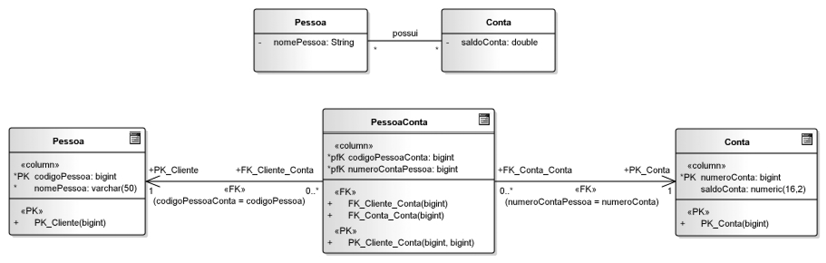
\includegraphics[width=0.95\columnwidth,height=0.35\textheight,keepaspectratio]{imagens/Fig4.60.png}
        \end{column}
        \begin{column}{0.5\textwidth}
            \textbf{Isolamento de Persistência:}
            \begin{itemize}
                \item \textbf{Padrão Repository (4.66):} Gerencia coleções de entidades em memória na camada de domínio.
                \item \textbf{Padrão DAO (4.68):} Encapsula comandos SQL e conexões com o SGBD na camada de persistência.
            \end{itemize}
            \centering
            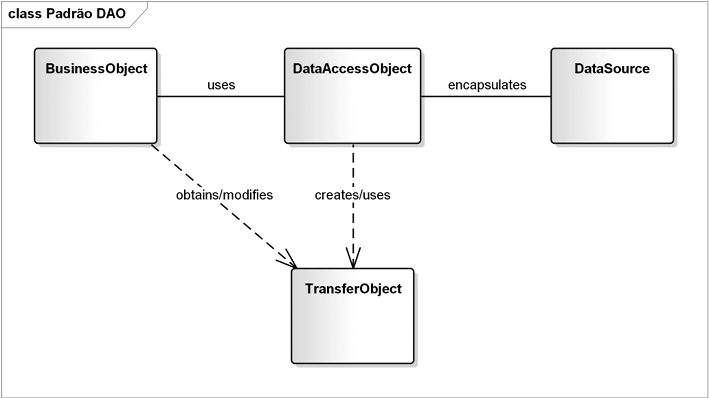
\includegraphics[width=0.95\columnwidth,height=0.42\textheight,keepaspectratio]{imagens/Fig4.68.png}
        \end{column}
    \end{columns}
\end{frame}

% -----------------------------------------------------------------------------
% SLIDE 19: Código Python de Apoio (exemplo_classes_atividades.py)
% -----------------------------------------------------------------------------
\begin{frame}[fragile]{Mapeamento em Python: Composição e Realização}
    Trecho do arquivo \texttt{exemplo\_classes\_atividades.py} (Figuras 4.11 e 4.18):
\begin{lstlisting}
class Edicao:
    def __init__(self, numero: int, volume: int, titulos_artigos: List[str]):
        self.numero_edicao = numero
        # Composicao forte (*--): Artigos instanciados e possuidos pela Edicao
        self.__artigos: List[Artigo] = [Artigo(t) for t in titulos_artigos]

class Pagamento(ABC):  # <<interface>> Pagamento (Figura 4.18)
    @abstractmethod
    def quitar_pedido(self, valor: float) -> str:
        pass

class PagamentoCartaoCredito(Pagamento):  # Realiza (implementa) Pagamento
    def quitar_pedido(self, valor: float) -> str:
        return f"Pagamento de R$ {valor:.2f} autorizado via Cartao de Credito."
\end{lstlisting}
\end{frame}

% =============================================================================
\section{Diagrama de Atividades: Fluxos e Processos (Cap. 10)}
% =============================================================================

% -----------------------------------------------------------------------------
% SLIDE 20: Introdução ao Diagrama de Atividades e Elementos Básicos
% -----------------------------------------------------------------------------
\begin{frame}{Diagrama de Atividades: Elementos Básicos (Cap. 10)}
    \begin{columns}
        \begin{column}{0.54\textwidth}
            \textbf{Finalidade do Diagrama de Atividades:}
            \begin{itemize}
                \item Modela a lógica procedural de um algoritmo, método, workflow de negócios ou fluxo de um Caso de Uso.
                \item Equivale aos antigos fluxogramas evoluídos para suportar orientação a objetos e concorrência!
            \end{itemize}
            \vspace{0.1cm}
            \textbf{Nós Fundamentais (Fig. 10.2 a 10.5):}
            \begin{itemize}
                \item \textbf{Nó Inicial ($\bullet$):} Disparo da atividade;
                \item \textbf{Nó de Ação:} Passo atômico de execução (retângulo arredondado);
                \item \textbf{Fluxo de Controle ($\longrightarrow$):} Transição entre ações;
                \item \textbf{Nó de Final de Atividade ($\odot$):} Término global da atividade.
            \end{itemize}
        \end{column}
        \begin{column}{0.46\textwidth}
            \centering
            \textbf{Nó Inicial e Ações (Fig. 10.4):}\\[0.1cm]
            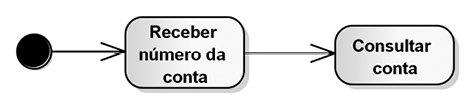
\includegraphics[width=0.95\columnwidth,height=0.22\textheight,keepaspectratio]{imagens/Fig10.4.png}\\[0.2cm]
            \textbf{Nó de Final de Atividade (Fig. 10.5):}\\[0.1cm]
            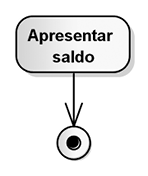
\includegraphics[width=0.85\columnwidth,height=0.22\textheight,keepaspectratio]{imagens/Fig10.5.png}
        \end{column}
    \end{columns}
\end{frame}

% -----------------------------------------------------------------------------
% SLIDE 21: Nó de Decisão, Guardas e Exemplo Emitir Saldo (Fig. 10.6 e 10.7)
% -----------------------------------------------------------------------------
\begin{frame}{Nó de Decisão, Condições de Guarda e Fluxo Completo}
    \begin{columns}
        \begin{column}{0.48\textwidth}
            \textbf{Nó de Decisão / Fusão (10.6):}
            \begin{itemize}
                \item Representado por um \textbf{losango ($\lozenge$)}.
                \item Divide o fluxo em caminhos alternativos mutuamente exclusivos.
                \item Cada saída é rotulada por uma \textbf{Condição de Guarda entre colchetes} (ex.: \texttt{[Conta válida]} vs. \texttt{[Conta inválida]}).
            \end{itemize}
            \vspace{0.15cm}
            \centering
            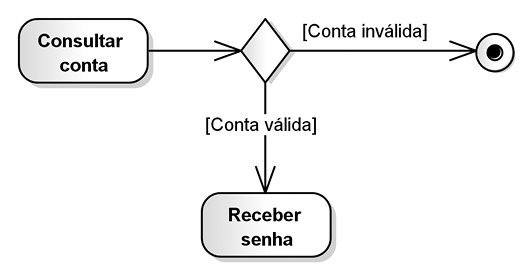
\includegraphics[width=0.95\columnwidth,height=0.32\textheight,keepaspectratio]{imagens/Fig10.6.png}
        \end{column}
        \begin{column}{0.52\textwidth}
            \centering
            \textbf{Atividade Emitir Saldo (Figura 10.7):}\\[0.08cm]
            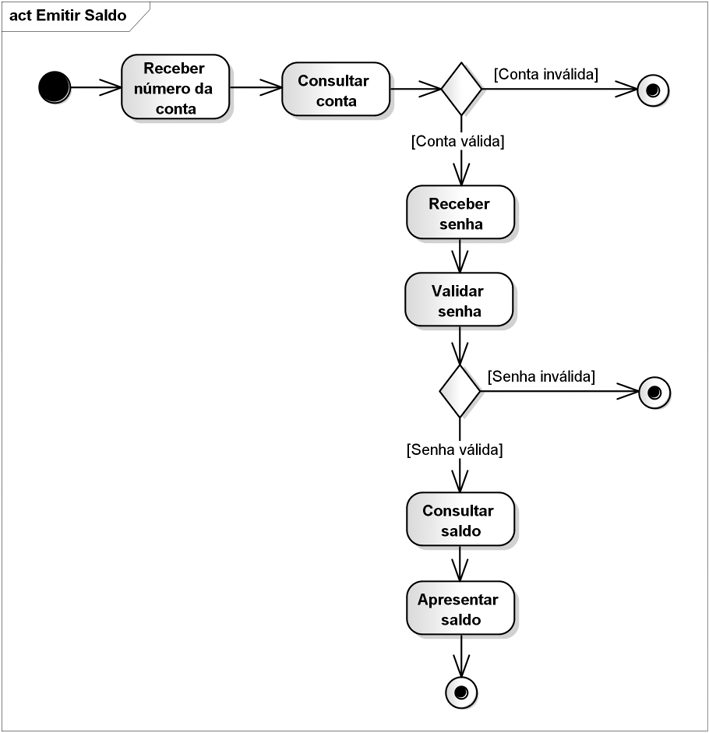
\includegraphics[width=\columnwidth,height=0.72\textheight,keepaspectratio]{imagens/Fig10.7.png}
        \end{column}
    \end{columns}
\end{frame}

% -----------------------------------------------------------------------------
% SLIDE 22: Paralelismo (Fork/Join) e Final de Fluxo (Fig. 10.8 e 10.9)
% -----------------------------------------------------------------------------
\begin{frame}{Paralelismo (Bifurcação/União) e Final de Fluxo}
    \begin{columns}
        \begin{column}{0.5\textwidth}
            \textbf{Barra de Bifurcação e União (10.8):}
            \begin{itemize}
                \item \textbf{Bifurcação (\textit{Fork}):} Barra espessa que divide 1 fluxo em 2 ou mais fluxos \textbf{concorrentes/paralelos}.
                \item \textbf{União (\textit{Join}):} Sincroniza e aguarda a conclusão de todos os ramos paralelos antes de prosseguir.
            \end{itemize}
            \centering
            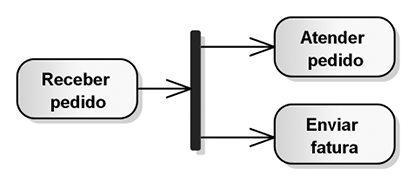
\includegraphics[width=0.95\columnwidth,height=0.42\textheight,keepaspectratio]{imagens/Fig10.8.png}
        \end{column}
        \begin{column}{0.5\textwidth}
            \textbf{Nó de Final de Fluxo ($\otimes$) (10.9):}
            \begin{itemize}
                \item Círculo contendo um \textbf{X}.
                \item Encerra \textbf{apenas o ramo paralelo local}, permitindo que as demais threads/ramos da atividade continuem executando!
            \end{itemize}
            \centering
            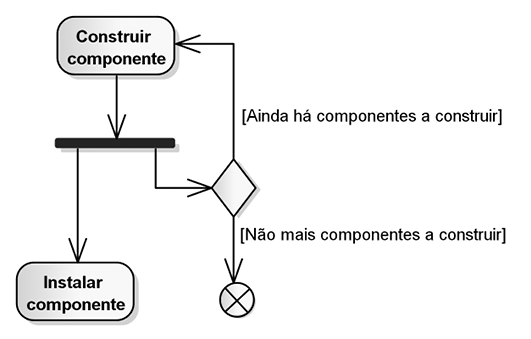
\includegraphics[width=0.95\columnwidth,height=0.45\textheight,keepaspectratio]{imagens/Fig10.9.png}
        \end{column}
    \end{columns}
\end{frame}

% -----------------------------------------------------------------------------
% SLIDE 23: Fluxo de Objetos, Nó de Objeto, Alfinetes e DataStore (10.10, 10.11, 10.13)
% -----------------------------------------------------------------------------
\begin{frame}{Fluxo de Objetos, Alfinetes (\textit{Pins}) e DataStore}
    \begin{columns}
        \begin{column}{0.5\textwidth}
            \textbf{Nó de Objeto e Estado (10.10):}
            \begin{itemize}
                \item Retângulo representando uma instância manipulada ou produzida por uma ação, podendo exibir seu estado entre colchetes (ex.: \texttt{ContaComum [Aberta]}).
            \end{itemize}
            \centering
            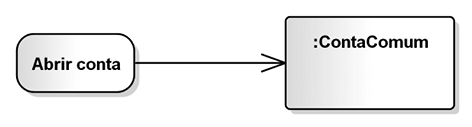
\includegraphics[width=0.92\columnwidth,height=0.28\textheight,keepaspectratio]{imagens/Fig10.10.png}\\[0.1cm]
            \textbf{Alfinetes / \textit{Pins} (10.11):}\\[0.05cm]
            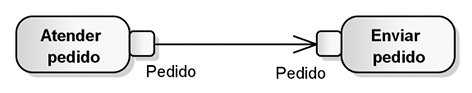
\includegraphics[width=0.92\columnwidth,height=0.22\textheight,keepaspectratio]{imagens/Fig10.11.png}
        \end{column}
        \begin{column}{0.5\textwidth}
            \textbf{Repositório de Dados (10.13):}
            \begin{itemize}
                \item Nó de objeto com estereótipo \texttt{<<datastore>>} que armazena dados de forma persistente durante a atividade.
            \end{itemize}
            \vspace{0.15cm}
            \centering
            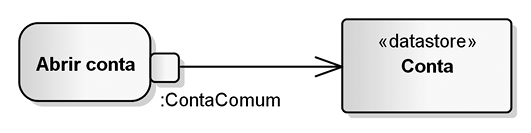
\includegraphics[width=0.95\columnwidth,height=0.45\textheight,keepaspectratio]{imagens/Fig10.13.png}
        \end{column}
    \end{columns}
\end{frame}

% -----------------------------------------------------------------------------
% SLIDE 24: Exceções, Sinais e Eventos Temporais (Fig. 10.14, 10.15, 10.16)
% -----------------------------------------------------------------------------
\begin{frame}{Tratamento de Exceções, Sinais e Eventos de Tempo}
    \begin{columns}
        \begin{column}{0.5\textwidth}
            \textbf{1. Fluxo de Interrupção / Exceção (10.14):}
            \begin{itemize}
                \item Seta em formato de \textbf{raio (zigue-zague)} ligando a ação geradora ao manipulador de exceção.
            \end{itemize}
            \centering
            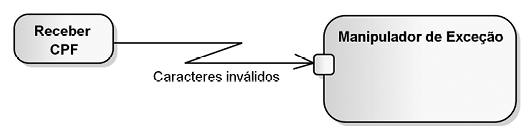
\includegraphics[width=0.92\columnwidth,height=0.28\textheight,keepaspectratio]{imagens/Fig10.14.png}\\[0.1cm]
            \textbf{2. Evento de Tempo / \textit{Timer} (10.16):}
            \begin{itemize}
                \item Símbolo de ampulheta (disparo temporal ou \textit{cron/trigger}).
            \end{itemize}
            \centering
            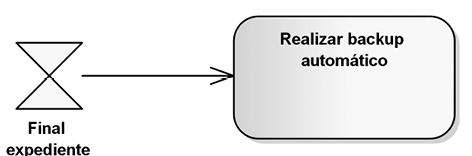
\includegraphics[width=0.88\columnwidth,height=0.22\textheight,keepaspectratio]{imagens/Fig10.16.png}
        \end{column}
        \begin{column}{0.5\textwidth}
            \textbf{3. Envio e Aceitação de Sinal (10.15):}
            \begin{itemize}
                \item \textbf{Envio de Sinal:} Polígono convexo (ponta para a direita);
                \item \textbf{Aceitação de Evento:} Polígono côncavo (reentrância à esquerda) que aguarda resposta assíncrona.
            \end{itemize}
            \vspace{0.1cm}
            \centering
            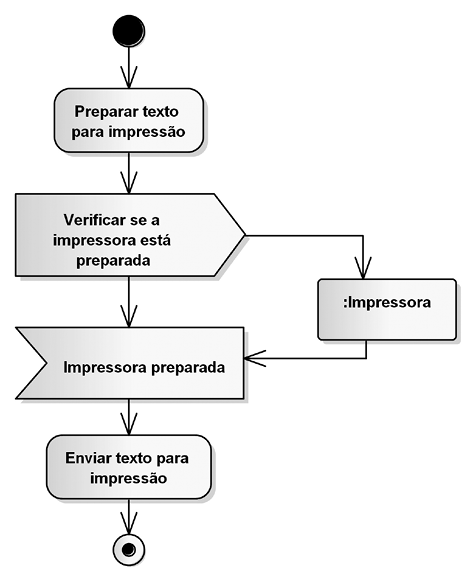
\includegraphics[width=0.95\columnwidth,height=0.46\textheight,keepaspectratio]{imagens/Fig10.15.png}
        \end{column}
    \end{columns}
\end{frame}

% -----------------------------------------------------------------------------
% SLIDE 25: Chamada de Comportamento e Operação (Fig. 10.17 e 10.18)
% -----------------------------------------------------------------------------
\begin{frame}{Chamada de Comportamento vs. Chamada de Operação}
    \begin{columns}
        \begin{column}{0.55\textwidth}
            \textbf{Ação de Chamada de Comportamento (10.17):}
            \begin{itemize}
                \item Invoca outra \textbf{Atividade já modelada} (símbolo de \textbf{ancinho/tridente} no canto inferior direito).
                \item Permite modularizar diagramas extensos reaproveitando subatividades (\textit{Consultar Conta}, \textit{Realizar Saque}).
            \end{itemize}
            \centering
            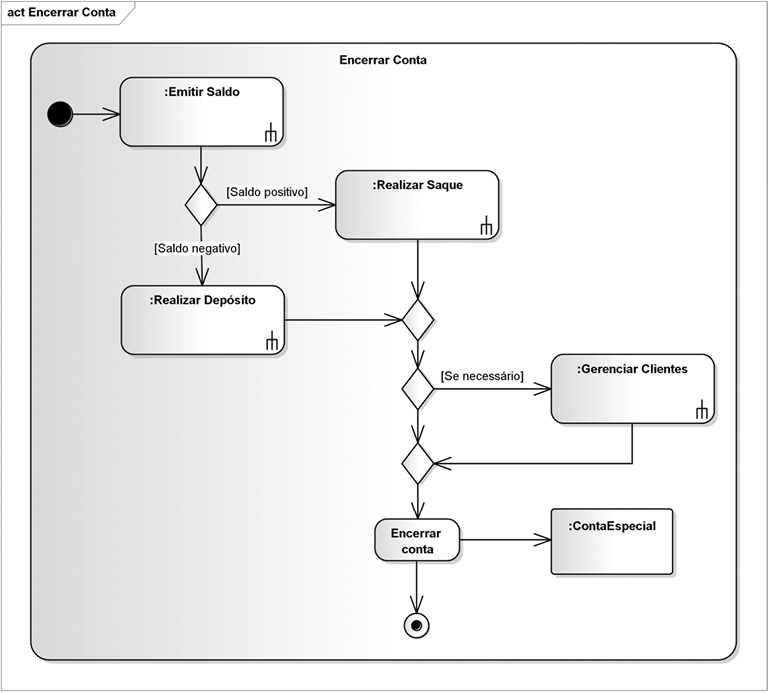
\includegraphics[width=0.95\columnwidth,height=0.48\textheight,keepaspectratio]{imagens/Fig10.17.png}
        \end{column}
        \begin{column}{0.45\textwidth}
            \textbf{Chamada de Operação (10.18):}
            \begin{itemize}
                \item Invoca diretamente um \textbf{método de uma classe} na notação \texttt{(Classe::metodo)}.
            \end{itemize}
            \vspace{0.2cm}
            \centering
            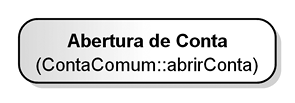
\includegraphics[width=0.88\columnwidth,height=0.35\textheight,keepaspectratio]{imagens/Fig10.18.png}
        \end{column}
    \end{columns}
\end{frame}

% -----------------------------------------------------------------------------
% SLIDE 26: Partições de Atividade / Swimlanes (Fig. 10.19)
% -----------------------------------------------------------------------------
\begin{frame}{Partições de Atividade (\textit{Swimlanes} / Raias de Natação)}
    \centering
    \textbf{Organização de Responsabilidades por Setor ou Ator (Figura 10.19):}\\[0.1cm]
    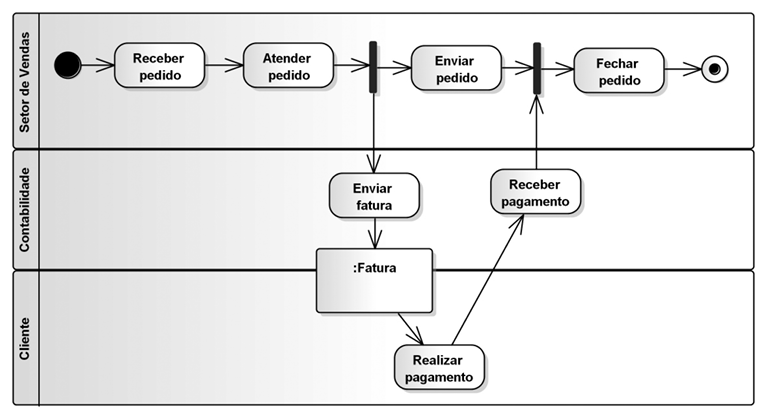
\includegraphics[width=0.94\textwidth,height=0.58\textheight,keepaspectratio]{imagens/Fig10.19.png}\\[0.08cm]
    \begin{block}{Importância Prática das Raias (\textit{Swimlanes})}
        \scriptsize Dividem visualmente a atividade em faixas horizontais ou verticais (\textbf{Setor de Vendas}, \textbf{Contabilidade}, \textbf{Cliente}), deixando explícito \textbf{quem é responsável} por executar cada ação do processo!
    \end{block}
\end{frame}

% -----------------------------------------------------------------------------
% SLIDE 27: Região Interrompível e Nós Estruturados (Fig. 10.20 e 10.23)
% -----------------------------------------------------------------------------
\begin{frame}{Região de Atividade Interrompível e Nós de Laço}
    \begin{columns}
        \begin{column}{0.54\textwidth}
            \textbf{Região Interrompível (Fig. 10.20):}
            \begin{itemize}
                \item Retângulo tracejado com bordas arredondadas envolvendo um grupo de ações.
                \item Se um evento de interrupção ocorrer (ex.: \textit{Cancelar pedido}), um fluxo em raio aborta imediatamente todas as ações internas da região.
            \end{itemize}
            \centering
            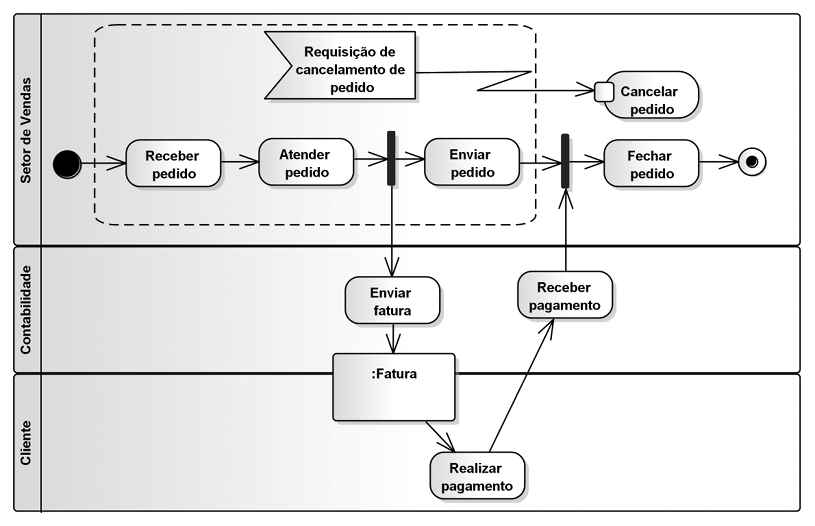
\includegraphics[width=0.96\columnwidth,height=0.45\textheight,keepaspectratio]{imagens/Fig10.20.png}
        \end{column}
        \begin{column}{0.46\textwidth}
            \textbf{Nó Estruturado de Laço (10.23):}
            \begin{itemize}
                \item Estereótipo \texttt{<<loop node>>} dividido em \textit{Setup} (iniciação), \textit{Teste} e \textit{Corpo} iterativo.
            \end{itemize}
            \vspace{0.1cm}
            \centering
            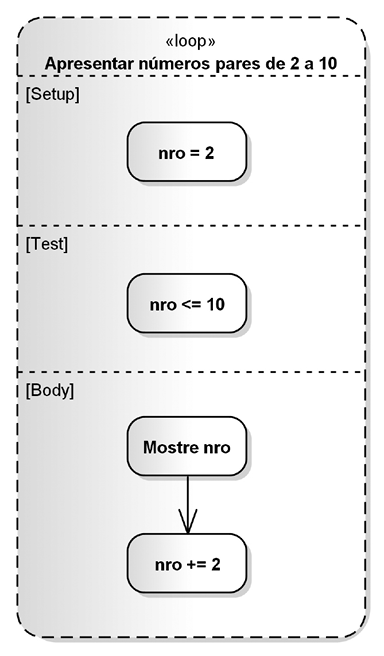
\includegraphics[width=0.95\columnwidth,height=0.48\textheight,keepaspectratio]{imagens/Fig10.23.png}
        \end{column}
    \end{columns}
\end{frame}

% -----------------------------------------------------------------------------
% SLIDE 28: Estudo de Caso Bancário: Realizar Saque (Fig. 10.28)
% -----------------------------------------------------------------------------
\begin{frame}{Estudo de Caso Bancário: Processo de Realizar Saque}
    \centering
    \textbf{Diagrama de Atividade Completo - Realizar Saque (Figura 10.28):}\\[0.1cm]
    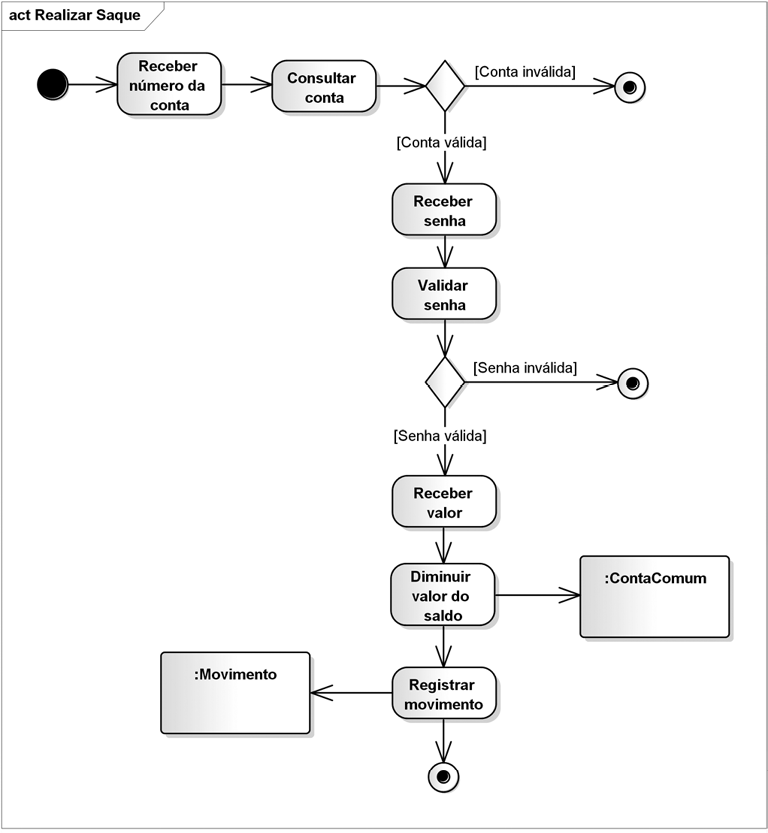
\includegraphics[width=0.92\textwidth,height=0.73\textheight,keepaspectratio]{imagens/Fig10.28.png}\\[0.08cm]
    \scriptsize Combina decisões de validação de conta/senha/saldo, chamada de comportamento e atualização dos objetos \texttt{ContaComum}, \texttt{ContaEspecial} e \texttt{Movimento}.
\end{frame}

% -----------------------------------------------------------------------------
% SLIDE 29: Estudo de Caso Web: Realizar Leilão Via Internet (Fig. 10.32)
% -----------------------------------------------------------------------------
\begin{frame}{Estudo de Caso Web: Processo de Realizar Leilão Online}
    \centering
    \textbf{Diagrama de Atividade - Sistema de Leilão Via Internet (Figura 10.32):}\\[0.1cm]
    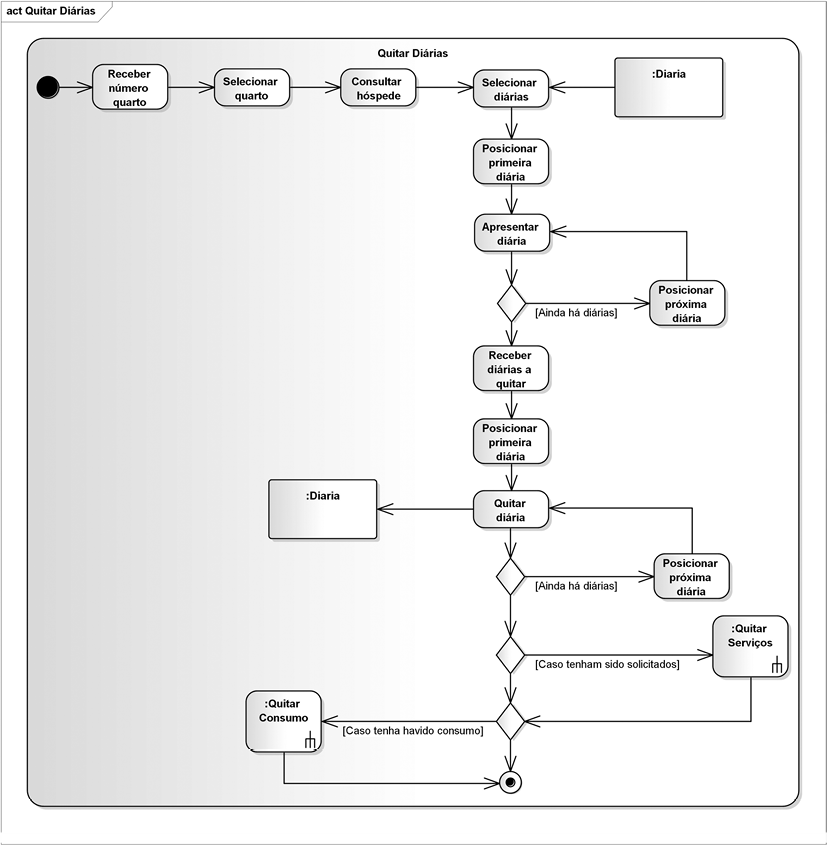
\includegraphics[width=0.92\textwidth,height=0.73\textheight,keepaspectratio]{imagens/Fig10.32.png}\\[0.08cm]
    \scriptsize Demonstra laços de recepção de lances, controle de tempo de anúncio e transição de estado do objeto \texttt{ItemLeilao [Arrematado]}.
\end{frame}

% =============================================================================
\section{Atividade Prática: TauáDelivery Web (Classes e Atividades)}
% =============================================================================

% -----------------------------------------------------------------------------
% SLIDE 30: Proposta da Atividade Prática
% -----------------------------------------------------------------------------
\begin{frame}{Atividade Prática: Estrutura e Fluxo do \textit{TauáDelivery Web}}
    \begin{block}{Continuidade do Projeto \textit{TauáDelivery Web}}
        Na Aula 20 modelamos os Casos de Uso (\textbf{RF01 a RF13}). Agora projetaremos o \textbf{Diagrama de Classes de Domínio} e o \textbf{Diagrama de Atividades com Raias}!
    \end{block}
    \vspace{0.15cm}
    \begin{columns}
        \begin{column}{0.5\textwidth}
            \textbf{Escopo do Diagrama de Classes:}
            \begin{itemize}
                \item Superclasse abstrata \texttt{UsuarioCadastrado} $\triangleleft$ \texttt{Cliente} e \texttt{Entregador};
                \item Composição: \texttt{Pedido} $\blacklozenge\to$ \texttt{ItemPedido} $\to$ \texttt{Produto};
                \item Enumeração \texttt{<<enumeration>> StatusPedido};
                \item Interface \texttt{<<interface>> Pagamento} realizada por \texttt{PagamentoPix} e \texttt{PagamentoCartaoCredito}.
            \end{itemize}
        \end{column}
        \begin{column}{0.5\textwidth}
            \textbf{Escopo do Diagrama de Atividades:}
            \begin{itemize}
                \item Processo \textbf{UC03 - Finalizar Pedido};
                \item \textbf{3 Partições (Raias):} Cliente, Sistema TauáDelivery e Gateway de Pagamento;
                \item Decisões de autenticação e aprovação financeira;
                \item Paralelismo (\textit{Fork/Join}) para notificar restaurante e emitir comprovante.
            \end{itemize}
        \end{column}
    \end{columns}
\end{frame}

% -----------------------------------------------------------------------------
% SLIDE 31: Exemplo Resolvido de Apoio 1: Diagrama de Classes
% -----------------------------------------------------------------------------
\begin{frame}{Exemplo de Apoio 1: Modelo de Classes do Cardápio}
    \centering
    \textbf{Subsistema de Cardápio (Modelo de Referência Resolvido):}\\[0.15cm]
    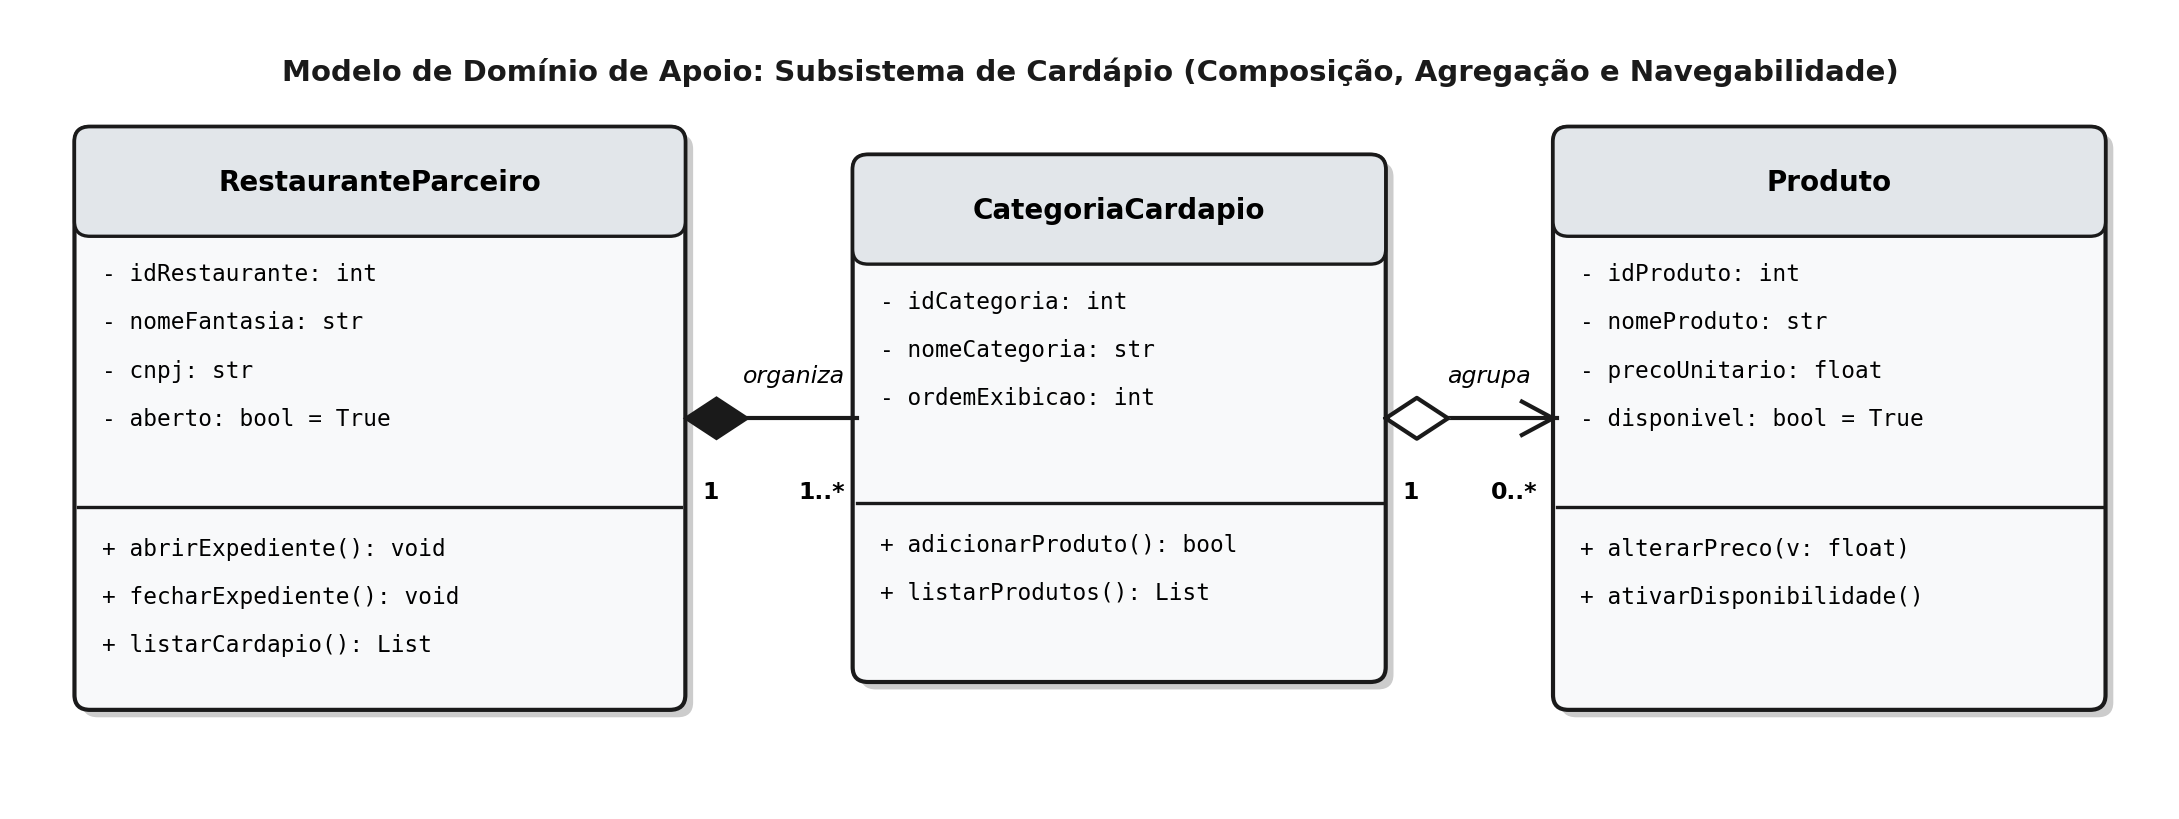
\includegraphics[width=0.95\textwidth,height=0.58\textheight,keepaspectratio]{imagens/modelagem_classes_apoio.png}\\[0.15cm]
    \begin{block}{Análise Técnica do Exemplo}
        \scriptsize \texttt{RestauranteParceiro} compõe (\textbf{$\blacklozenge$}) suas \texttt{CategoriaCardapio} (\texttt{1} para \texttt{1..*}), enquanto cada categoria agrega (\textbf{$\lozenge$}) e navega para os objetos \texttt{Produto} (\texttt{1} para \texttt{0..*}).
    \end{block}
\end{frame}

% -----------------------------------------------------------------------------
% SLIDE 32: Exemplo Resolvido de Apoio 2: Diagrama de Atividades
% -----------------------------------------------------------------------------
\begin{frame}{Exemplo de Apoio 2: Diagrama de Atividades do Carrinho}
    \centering
    \textbf{Fluxo com Partições para UC02 - Gerenciar Carrinho (Modelo de Apoio):}\\[0.15cm]
    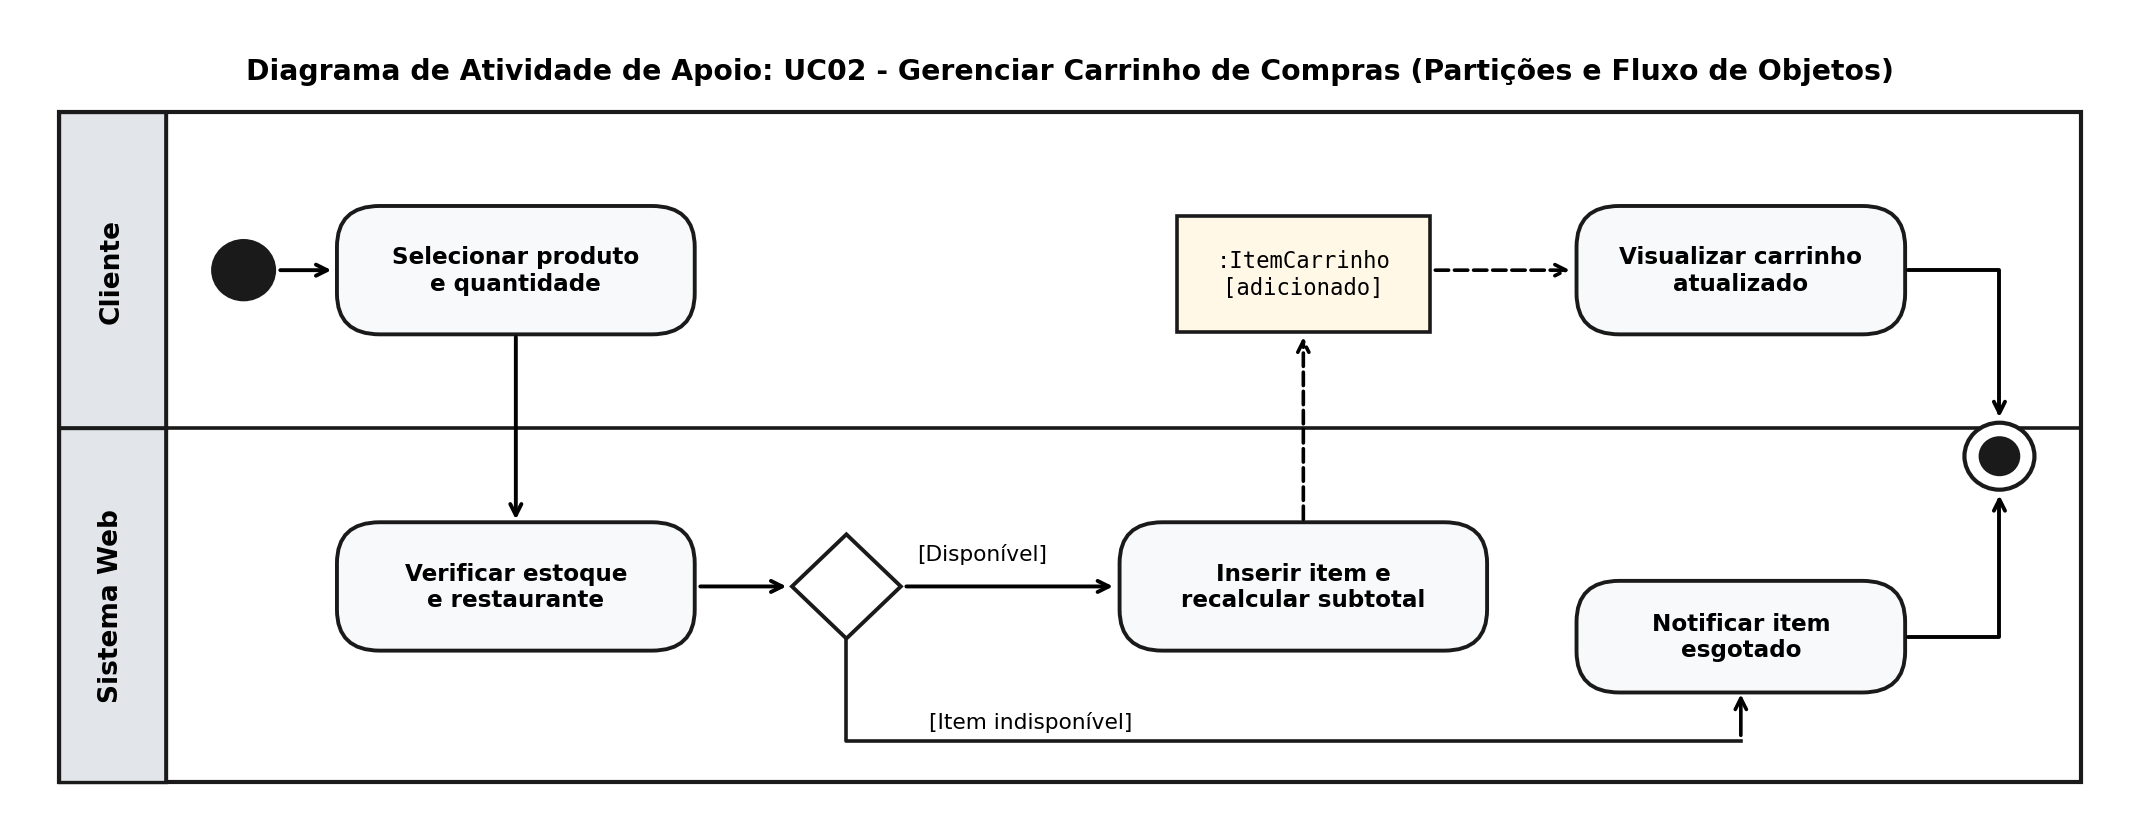
\includegraphics[width=0.95\textwidth,height=0.58\textheight,keepaspectratio]{imagens/modelagem_atividade_apoio.png}\\[0.15cm]
    \begin{block}{Análise Técnica do Exemplo}
        \scriptsize Separa claramente as ações das raias \textbf{Cliente} e \textbf{Sistema Web}, aplicando Nó de Decisão com guardas \texttt{[Disponível]} / \texttt{[Item indisponível]} e Fluxo de Objetos \texttt{:ItemCarrinho [adicionado]}.
    \end{block}
\end{frame}

% -----------------------------------------------------------------------------
% SLIDE 33: Entregáveis da Atividade Prática
% -----------------------------------------------------------------------------
\begin{frame}{Roteiro de Entrega da Atividade Prática}
    \begin{columns}
        \begin{column}{0.5\textwidth}
            \begin{block}{Parte 1: Questões Conceituais (3,0 pts)}
                \footnotesize
                \begin{itemize}
                    \item Diferença de ciclo de vida entre Agregação ($\lozenge$) e Composição ($\blacklozenge$);
                    \item Classe Associativa vs. Classe Intermediária para avaliações de pedidos;
                    \item Vantagem do polimorfismo com \texttt{<<interface>> Pagamento};
                    \item Nó de Decisão vs. Barra \textit{Fork/Join} e Final de Atividade vs. Final de Fluxo.
                \end{itemize}
            \end{block}
        \end{column}
        \begin{column}{0.5\textwidth}
            \begin{exampleblock}{Partes 2 e 3: Modelagem Visual (7,0 pts)}
                \footnotesize
                \begin{itemize}
                    \item \textbf{Parte 2 (4,0 pts):} Diagrama de Classes completo de Pedidos, Entregas e Pagamentos com multiplicidades, visibilidades e atributos derivados (\texttt{/}).
                    \item \textbf{Parte 3 (3,0 pts):} Diagrama de Atividades com 3 raias para o processo \textit{UC03 - Finalizar Pedido}.
                \end{itemize}
            \end{exampleblock}
        \end{column}
    \end{columns}
    \vspace{0.2cm}
    \begin{alertblock}{Dica de Ouro}
        Consultem o arquivo \texttt{atividade\_pratica.md} e executem \texttt{python3 exemplo\_classes\_atividades.py} para validar os conceitos em código!
    \end{alertblock}
\end{frame}

% -----------------------------------------------------------------------------
% SLIDE 34: Conclusão e Próxima Aula
% -----------------------------------------------------------------------------
\begin{frame}{Conclusão e Próximos Passos}
    \begin{itemize}
        \item \textbf{O Diagrama de Classes materializa a arquitetura estática:} Define com rigor a hierarquia, o acoplamento todo-parte (agregação/composição), os contratos de interface e o mapeamento relacional.
        \item \textbf{O Diagrama de Atividades governa o fluxo dinâmico:} Transforma especificações textuais de casos de uso em fluxos visuais precisos com decisões, paralelismo e raias de responsabilidade.
    \end{itemize}
    \vspace{0.3cm}
    \begin{exampleblock}{Próxima Aula (Aula 22)}
        \textbf{Diagramas de Interação e Máquina de Estados (Capítulos 7, 8 e 9):}
        Diagrama de Sequência (troca cronológica de mensagens e \textit{lifelines}), Diagrama de Comunicação e ciclo de vida de objetos com Máquina de Estados.
    \end{exampleblock}
\end{frame}

\end{document}
